\chapter{Concetti chiave}
\section{Terminologia di base}
Di seguito viene riportata un po' di terminologia tipica dell'ambito della 
cybersecurity.

\textbf{Asset}: è una risorsa che intendiamo proteggere, in questo corso faremo
più specificamente riferimento a dati, codice sorgente e proprietà intellettuale
come assets principali.

\textbf{Triade CIA}: L'obiettivo della cybersecurity è garantire la riservatezza,
l'integrità e la disponibilità (triade CIA) degli assets contro varie minacce.

\begin{itemize}
    \item \textbf{Confidenzialità}: La proprietà che le informazioni non siano rese
    disponibili o svelate ad individui, entità o processi non autorizzati. Al
    centro di questa definizione trovo l'informazione. Terze parti è un termine generico che
    viene declinato in individui, entità o processi.
    \item \textbf{Integrità}: La proprietà che i dati non siano stati modificati, distrutti
    o persi in modo non autorizzato o accidentale.
    \item \textbf{Disponibilità}: La proprietà di un sistema e delle sue risorse di essere 
    accessibili e di performare rispettando le specifiche per cui è stato progettato.
\end{itemize}

\textbf{Threat}: un'azione o un evento potenzialmente negativo (accidentale o 
intenzionale) causato da una vulnerabilità che comporta un impatto indesiderato
su un sistema informatico o un'applicazione. Chi sono gli attori dietro un Threat
intenzionale?

\begin{itemize}
    \item \textbf{State-sponsored}: agenzie sponsorizzate dagli stati, sono 
    organizzazioni governative. Cyberattacchi che hanno lo scopo di mettere in
    difficoltà uno stato nemico. Il DDoS è in genere l'attacco più comune ma non è il 
    solo, ci sono altri attacchi come i wiper (distrugge le informazioni su un pc), 
    creare disinformazione, ecc. Un esempio di attacco condotto da organizzazioni
    state-sponsored è \textit{NotPetya} il quale sfruttava una vulnerabilità di Windows
    (\textit{Eternal Blue}) per infettare i dispositivi target. In genere i Threats di questa
    categoria sono definiti \textbf{persistenti} poichè i malware cercano di 
    espandersi nella rete quanto più velocemente e, spesso, silenziosamente possibile.
    Molto spesso gli stati nemici dello stato attaccante sono già stati ingettati
    da malware, lo stato attaccante quindi aspetterà solo il momento giusto per far
    "esplodere" il virus.
    \item \textbf{Cybercriminali}: gruppi di persone motivate da uno scopo economico. 
    Monetizzano gli attacchi rubando dati privati come carte di credito e 
    vendendoli ad esempio sul dark web oppure chiedendo direttamente un 
    riscatto alla vittima.
    \item \textbf{Hacktivisti}: gruppi di persone motivati da ideali politici, 
    sociali, religiosi, economici, ambientali, ecc. 
    \item \textbf{Hackers-for-hire}: hacker che lavorano per altri gruppi di 
    attaccanti. Ad esempio si può trattare di persone che scrivono effettivamente 
    il malware per poi venderlo ad altri gruppi che eseguono l'attacco. Il 
    loro modello di business permette loro di prendere le distanze dai reati 
    commessi dai loro clienti.
\end{itemize}

\textbf{Vulnerabilità}: L'esistenza di una debolezza, di un errore di 
progettazione o di implementazione che può portare a un evento imprevisto e 
indesiderato che compromette la sicurezza del sistema informatico, della rete, 
dell'applicazione o del protocollo in questione. Possiamo distinguere quattro 
tipi di vulnerabilità:

\begin{itemize}
    \item Vulnerabilità di \textbf{design}: un'applicazione pensata male, come 
    molti protocolli storicamente usati nelle reti.
    \item Vulnerabilità \textbf{software}: si tratta di errori di programmazione
    (bug), tali errori possono portare ad effetti noti come: buffer overflow, race 
    conditions, input validation non corretta o mancante.
    \item Vulnerabilità di \textbf{misconfigurazione}: si tratta di configurazione 
    errata dei sistemi, spesso perchè si lasciano alcune opzioni di default in 
    applicazioni molto complesse (come \textit{WordPress}).
    \item Vulnerabilità dovute agli \textbf{umani}: esempi noti riguardano una
    gestione inadeguata delle password, utilizzo di software obsoleto o non autorizzato,
    clic su link e allegati sospetti, ecc.
\end{itemize}

\textbf{Attack vector}: Un vettore di attacco è un percorso o un mezzo 
attraverso il quale un aggressore può ottenere l'accesso a un computer per 
eseguire un codice dannoso (\textbf{payload}) o causare un danno. Esempi 
di vettori di attacco sono: e-mail dannose, allegati, worm, pagine web, download, inganni
(noti anche come \textit{ingegneria sociale}), una shell locale.

\textbf{Exploit}: Un exploit è un programma, un blocco di dati o una sequenza di
comandi che sfrutta una vulnerabilità.

\textbf{Zero day}: Lo zero day è proprio quella finestra temporale in cui un 
attaccante scopre la vulnerabilità, il vendor scopre successivamente la 
presenza della vulnerabilità e deve quindi ricorrere ai ripari (la finestra 
termina proprio quando il vendor rilascia la patch che fixa la vulnerabilità). 

\begin{figure}[H]
    \centering
    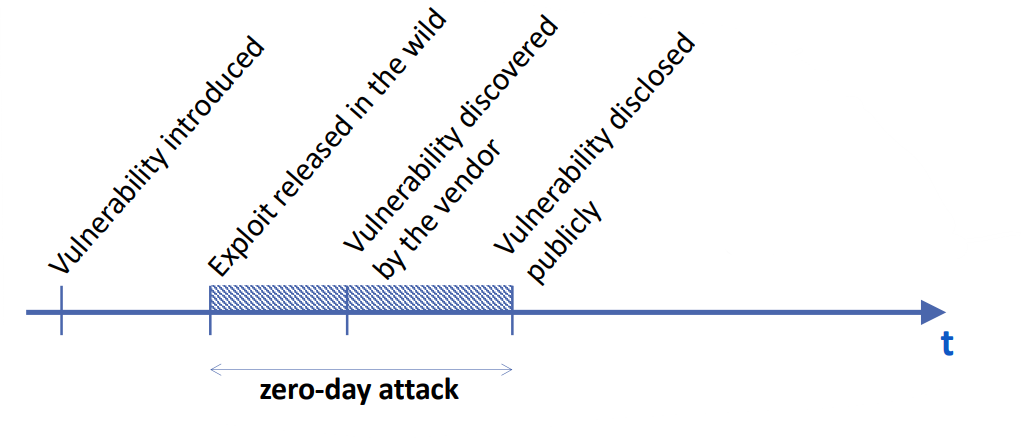
\includegraphics[width=1.0\linewidth]{img/capitolo1/zeroday.png}
    \label{fig:zeroday}
\end{figure}

Le vulnerabilità zero-day sono quindi sconosciute ai responsabili della 
sicurezza e non esistono misure di mitigazione disponibili. D'altro canto le 
vulnerabilità note possono essere comunque sfruttate anche dopo la loro individuazione, 
sebbene con un impatto minore.

\section{CVE}
Le vulnerabilità vengono rese pubbliche online. Per evitare duplicazioni di 
lavoro e consentire la condivisione dei dati, il MITRE ha introdotto il 
sistema Common Vulnerabilities and Exposures (\textbf{CVE}).

Si tratta di un database popolato da tantissime vulnerabilità scoperte. Ogni 
volta che qualcuno trova una nuova vulnerabilità si procede ad associarle un 
identificativo e l'anno in cui essa è stata scoperta.

\begin{gather*}
    \text{Formato: CVE-YEAR-NUMBER} \\
    \text{Esempio: CVE-2014-0160 ("Heartbleed")}
\end{gather*}

Nell'esempio riportato vediamo la vulnerabilità nota come \textit{Heartbleed}: si
tratta di una vulnerabilità di tipo buffer overflow che riguardava OpenSSL v.1.0.1.
Essa è stata dunque registrata dal CVE nel 2014 con identificativo 0160.

Ciascuna istanza CVE include le seguenti informazioni:

\begin{itemize}
    \item Una descrizione della vulnerabilità
    \item Un punteggio CVSS (gravità della vulnerabilità)
    \item Un CWE (il tipo o la famiglia della vulnerabilità)
    \item Un elenco di CPE (prodotti interessati dal CVE)
    \item Riferimenti (link a exploit "proof-of-concept", bollettini dei fornitori)
\end{itemize}

\subsection{CVSS}

Il Common Vulnerability Scoring System (\textbf{CVSS}) è un sistema utilizzato per 
quantificare la gravità di una vulnerabilità. La scala va da 1 a 10. 
Ci sono vari criteri per stabilire questo punteggio: 

\textbf{Base Metric Group}: “intrinseca” gravità della vulnerabilità,
indipendentemente dalla sua data di insorgenza e dai sistemi di destinazione.
Qui si valuta il vettore di attacco (Network, Adiacente, Locale, Fisico), la 
complessità dell'attacco, i requisiti, i privilegi richiesti e l'interazione
utente necessaria.

\textbf{Threat Metric Group}: (opzionale) si valuta lo stato attuale delle 
tecniche di exploit o la disponibilità di codice per una vulnerabilità. 
Chiaramente più è facile sfruttare una vulnerabilità, più alto è il punteggio 
di vulnerabilità.

\textbf{Environmental Metric Group}: (opzionale) gli analisti possono 
personalizzare il punteggio in base all'importanza delle risorse IT interessate
e ai controlli di sicurezza in atto. Si cerca di quantificare la perdita dei requisiti
richiesti dalla triade CIA, quindi si valuta la vulnerabilità in termini di perdita
di Confidenzialità, Integrità e Disponibilità.

Una volta ottenuti i punteggi dei Threat ed Environmental group, questi vengono
combinati con lo score del Base group al fine di ottenere il punteggio di gravità
definitivo.

\subsection{CWE}

Il \textbf{CWE} definisce un elenco di tipi di vulnerabilità (ovvero una 
categoria di vulnerabilità).

\begin{gather*}
    \text{CWE-120: Buffer Copy without Checking Size of Input}
\end{gather*}

Nell'esempio riportato capiamo quindi che con l'identificativo 120 andiamo a 
riferirci a tutte quelle vulnerabilità di tipo buffer overflow.

\subsection{CPE}

Il \textbf{CPE} è uno schema di denominazione strutturato per prodotti hardware e software.
Denominare con un nome standard un prodotto non è affatto banale in quanto spesso
lo stesso prodotto può avere più nomi creando così possibile ambiguità.

\begin{gather*}
    \text{Microsoft Windows 7 64-bit Service Pack 1}\\
    \text{cpe:/o:microsoft:windows\_7:-:sp1:x64}
\end{gather*}

Dove la "o" sta ad indicare che il prodotto in questione è un sistema operativo,
altre tipologie di prodotto vengono indicate con "a" nel caso di applicazione, "h"
nel caso di hardware.

\section{Divulgazione delle vulnerabilità}

Non esiste un approccio “perfetto” alla divulgazione delle vulnerabilità dato 
che tale processo coinvolge molte parti con interessi contrastanti. Prima tra 
tutti troviamo i \textbf{Vendors} i quali vogliono che la divulgazione avvenga solo dopo
aver patchato la vulnerabilità, gli \textbf{Users} chiaramente vorrebbero che le patch 
arrivino il prima possibile, infine i \textbf{Researchers} pubblicano velocemente
le vulnerabilità scoperte per ottenere credito e per motivare i Vendors a rilasciare
le dovute patch.

Vediamo le diverse tipologie di divulgazioni possibili:

\textbf{Full disclosure}: Le vulnerabilità vengono divulgate il più velocemente
possibile, senza restrizioni. In questo scenario i Researchers non si coordinano
con i Vendors quindi le vittime potenziali (Users) ne sanno tanto quanto chi potrebbe attaccarle.

\textbf{Vendor disclosure}: Le vulnerabilità vengono divulgate verso i Vendors dai
Researchers, ovviamente l'obiettivo del Researcher è anche quello di avere un compenso
economico.

\textbf{Coordinated disclosure}: Le vulnerabilità vengono divulgate verso i Vendors
dai Researchers; i Vendors hanno una finestra temporale (tipicamente 60-120 giorni)
per fixare la vulnerabilità. Allo scadere della finestra temporale i Researchers
divulgano pubblicamente la vulnerabilità.
Ci possono essere altre entità che fanno da tramite in questo processo, da citare
sono le \textbf{CSIRTs} (Computer Security Incident Response Teams) che fanno appunto da mediatore tra Vendors e Researchers.

\textbf{Non-disclosure}: Le vulnerabilità non vengono divulgate verso gli Users/Vendors,
potrebbero piuttosto essere vendute a terze parti.